\documentclass[11pt]{beamer}

\usetheme{Darmstadt}

\usepackage{times}
\usefonttheme{structurebold}

\usepackage[english]{babel}
\usepackage{pgf,pgfarrows,pgfnodes,pgfautomata,pgfheaps}
\usepackage{amsmath,amssymb}
\usepackage[latin1]{inputenc}
\usepackage{multicol}

\input{slabbrev}

\title{Multivariate and Functional Principal Components without Eigenanalysis}

\author{Jim Ramsay, McGill University \\
      Workshop on Registration \\
      Mathematical Biosciences Institute \\
      Columbus, OH
      13 November 2012}
\date{}

\begin{document}

\begin{frame}

\maketitle

\end{frame}

%  ---------------------------------------------------------------------
%  ---------------------------------------------------------------------

\section{Overview}

%  --------------------------------------------------------------------

\begin{frame}

\frametitle{PCA: The essential idea}

\bi
  \item We have a $N$ by $n$ data matrix $\Xbold$.
  \item We propose the reduced rank $K$ bilinear model
  \[
    \Xbold = \Fbold \Abold
  \]
  where
    \bi
      \item $\Abold$ is a $K$ by $n$ matrix of principal component coefficients, with $K << n$
      \item $\Fbold$ is a $N$ by $K$ matrix of principal component scores
    \ei
  \item Usually $N >> n$, and the factor scores are interesting, but it's $\Abold$ that tells
  us what the core $K$ components of variation are, to within a full rank linear transformation.
  \item The fundamental goal of PCA is to identify a linear subspace $\cal{R}^K$.
\ei

\end{frame}

%  --------------------------------------------------------------------

\begin{frame}

\frametitle{What I'd like to do with PCA}

\bi
  \item Provide GLM capability: PCA for mixtures of types of variables, using fitting criteria
  appropriate to each data type.
  \item Define a fitting strategy that recognizes PC scores $\Fbold$ as nuisance parameters
  and PC components in $\Abold$ as structural parameters.
  \item Generalize PCA:
    \bi
      \item synthesize the treatment of both multivariate and functional data
      \item implement partial least squares: an approximation of an external vector $\ybold$ via a $K$ dimensional subspace $\cal{R}^K$
      \item combine PCA with the registration of functional data
    \ei
\ei

\end{frame}

%  ---------------------------------------------------------------------
%  ---------------------------------------------------------------------

\section{Beyond Eigenanalysis}

%  --------------------------------------------------------------------

\begin{frame}

\frametitle{Eigenanalysis and PCA}

\bi
  \item The singular value decomposition yields both $\Abold$ and $\Fbold$,
  \item But the usual procedure is to extract $\Abold$ from the eigenanalysis of $N^{-1} \Xbold' \Xbold$
  or the correlation matrix $\Rbold$
  \item and then use regression analysis to obtain the least squares estimate
  \[
    \Fbold = \Xbold \Abold' (\Abold' \Abold)^{-1}
  \]
\ei

\end{frame}

%  --------------------------------------------------------------------

\begin{frame}

\frametitle{Why eigenanalysis gets in the way}

\bi
  \item Eigenanalysis forces us to use least squares fitting for all variables.
  \item Eigenanalysis treats the estimation of $\Fbold$ and $\Abold$ symmetrically, but $\Abold$ contains structural parameters and $\Fbold$ contains nuisance parameters.  They require different estimation strategies.
  \item Eigenalysis inappropriately highlights the basis system rather than the subspace that it defines.
  \item Eigenalysis cannot accommodate extensions such as registration of functional data.
\ei

\end{frame}

%  ---------------------------------------------------------------------
%  ---------------------------------------------------------------------

\section{Parameter Cascading}

%  --------------------------------------------------------------------

\begin{frame}

\frametitle{Structural versus nuisance parameters}

\bi
  \item Nuisance parameters are required in a model to capture important variation, but are seldom themselves of direct interest.  A well-known example are random effect parameters in a mixed effects (ME) model.
  \item The number of nuisance parameters often depends on the configuration or design of the data.
  \item Structural parameters are typically of direct interest, for example fixed effect parameters for ME models.
  \item Their number is usually fixed, and typically much smaller than the number of nuisance parameters.
  \item Estimating nuisance and structural parameters using the same strategy risks burning up large number of degrees of freedom and rendering the structural parameter estimates unnecessarily unstable.  ME model estimation recognizes this.
\ei

\end{frame}

%  --------------------------------------------------------------------

\begin{frame}

\frametitle{The parameter cascading strategy}

\bi
  \item Parameter cascading is a method for estimating large and varying numbers of nuisance parameters $\cbold$ in the presence of a small fixed number of structural parameters $\thetabold$.
  \item Parameter cascading defines nuisance parameters as \emph{smooth} functions $\cbold(\thetabold)$ of structural parameters.
  \item Imposing smoothness or regularizing $\cbold(\thetabold)$ keeps nuisance parameters from burning up large numbers of degrees of freedom, and therefore stabilizes the structural parameter estimates.
  \item Nuisance parameter function $\cbold(\thetabold)$ is often defined by an inner optimization of a criterion $J(\cbold|\thetabold)$ each time $\thetabold$ is changed in an outer optimization cycle.
  \item The outer optimization $H(\thetabold)$ is frequently different from $J(\cbold|\thetabold).$
\ei

\end{frame}

%  --------------------------------------------------------------------

\begin{frame}

\frametitle{The parameter cascading strategy and the Implicit Function Theorem}

\bi
  \item The total derivative or gradient of $H$ with respect to $\thetabold$ requires the use of the Implicit Function Theorem:
    \[
        \frac{dH}{d \thetabold} = \frac{\partial H}{\partial \thetabold} -
        \frac{\partial H}{\partial \cbold} \bigg[\frac{\partial^2 J}{\partial^2 \cbold^2}\bigg]^{-1}
        \frac{\partial^2 J}{\partial \cbold \partial \thetabold}
    \]
  \item The total Hessian is also available in this way.
\ei

\end{frame}

%  ---------------------------------------------------------------------
%  ---------------------------------------------------------------------

\section{Parameter cascading for PCA}

%  --------------------------------------------------------------------

\begin{frame}

\frametitle{The parameter cascading strategy for multivariate PCA}

\bi
  \item We add smoothness to the least squares criterion for $\Fbold$ given $\Abold$ by attaching penalty terms:
  \[
    J(\Fbold|\Abold,\Xbold) = \| \Xbold - \Fbold \Abold) \|^2 +
              \lambda_1 \| \Fbold' \Pbold_1 \Fbold \|^2 + \lambda_2 \| \Fbold  \Pbold_2 \Fbold' \|^2.
  \]
  \item The minimizer $\hat{\Fbold}(\Abold)$ has a closed form expression.
  \item Order $K$ matrix $\Pbold_1$ and order $N$ matrix $\Pbold_2$ are often projectors onto complements of some pre-defined subspaces or special patterns.
  \item Smoothing parameters $\lambda_1 \geq 0$ and $\lambda_2 \geq 0$ allow us to control the emphasis that we place on the PC scores having these particular structures.
\ei

\end{frame}

%  --------------------------------------------------------------------

\begin{frame}

\frametitle{The fitting criterion for $\Abold$}

\bi
  \item This is defined in terms of only the PC coefficients $\Abold$.
  \item Consequently, we can choose our fitting criteria freely, such as
    \[
      H(\Abold) = -\sum_j^n \ln L_j(\Abold|\xbold_j)
    \]
  where $-\ln L_j$ is the negative log likelihood appropriate to variable $j$ and defined by data $N$-vector $\xbold_j$.
  \item The gradient of $G$ will depend on $\Abold$ both directly through its the partial derivative, and also via the $N$ functions $\fbold_i(\Abold)$
    \[
        \frac{dH}{d \Abold} = \frac{\partial H}{\partial \Abold} +
        \sum_i^N \frac{\partial H}{\partial F_i} \frac{dF_i}{d \Abold}
    \]
  \item PCA is now estimates $Kn$ parameters instead of $K(N+n)$ parameters.
\ei

\end{frame}

%  --------------------------------------------------------------------

\begin{frame}

\frametitle{Evaluating the fit}

\bi
  \item Without regularization, $\Abold$ and $\Fbold$ are defined to within a nonsingular linear transformation $\Wbold$ of order $K$: $\Fbold \Wbold \Wbold^{-1} \Abold$ provides the same fit to the data.
  \item Regularization may remove some of this unidentifiability, but some will inevitably remain.
  \item Consequently, we cannot assess fit in term of $\Abold$, but must rather focus our attention on:
  \bi
    \item predictive criteria assessing fit at the data level
    \item geometric measures of conformity between the $K$-dimensional estimated subspace and some true or population subspace.
  \ei
  \item Canonical correlation methodology serves these purposes well.
\ei

\end{frame}

%  --------------------------------------------------------------------

\begin{frame}

\frametitle{A simulated data example}

\bi
  \item $N = 200, n = 5, K = 2$, $\Fbold$ contains 200 equally spaced points on a circle, $\Abold = [[1,1,1,1,1];[-2,-1,0,1,2]]$  $\Xbold = \Fbold \Abold$ plus i.i.d. Gaussian error, $\sigma = 0.5.$
  \item The unregularized fit to the data yielded squared canonical correlations $\rho_1^2 = 0.99991$ and $\rho_2^2 = 0.99775$ between the true and estimated subspaces.
  \item The following figure compares unregularized and regularized estimates of $\Fbold$ where the regularization
  penalized departure from the true values.
\ei

\end{frame}

%  --------------------------------------------------------------------

\begin{frame}

\begin{center}
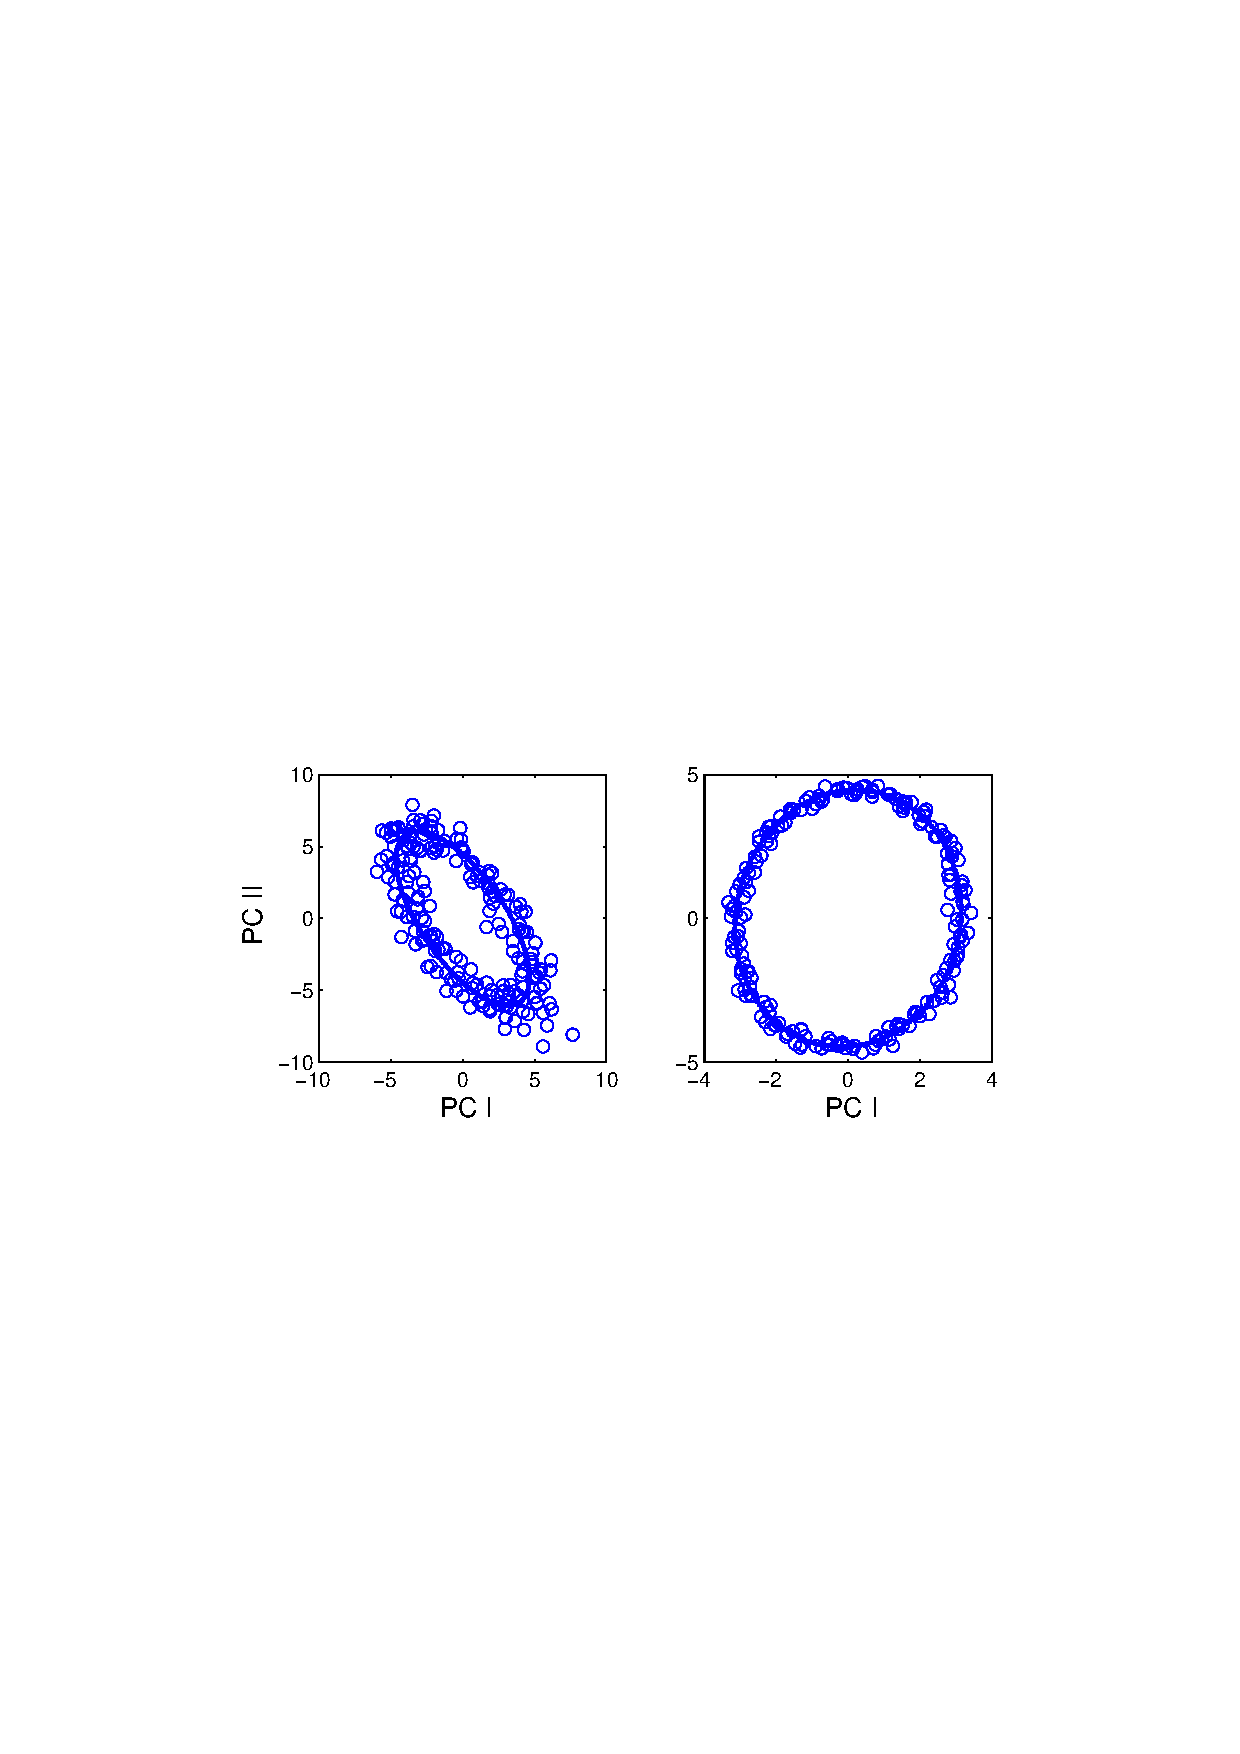
\includegraphics[width=4in]{figs/MDA1.png}
\end{center}

\end{frame}

%  --------------------------------------------------------------------

\begin{frame}

\frametitle{The parameter cascading strategy for functional PCA}

\bi
  \item The data are now $N$ functions $x_i(t)$
  \item The principal coefficients are now functions $a_k(t), k=1,\ldots,K$.
  \item The inner criterion $J$ is now:
  \[
    J(\Fbold|\abold,\xbold) = \sum_i \int [x_i(t) - \sum_k f_{ik} a_k(t)]^2 dt +
              \lambda_1 \| \Fbold' \Pbold_1 \Fbold \|^2 + \lambda_2 \| \Fbold  \Pbold_2 \Fbold' \|^2.
  \]
  \item Structural parameter $\Abold$ is now a $K$ by $L$ matrix of coefficients for a basis function of each $a_k$ in terms of $L$ basis functions.
\ei

\end{frame}

%  --------------------------------------------------------------------

\begin{frame}

\bi
  \item The outer criterion could be
  \[
    H(\Abold|\xbold) = \sum_i \int [x_i(t) - \sum_k f_{ik} a_k(t)]^2 dt + \lambda_3 \trace(\Abold \Ubold \Abold')
  \]
  where penalty matrix $\Ubold$ defines a roughness penalty for the $a_k$'s.
\ei

\end{frame}

%  ---------------------------------------------------------------------
%  ---------------------------------------------------------------------

\section{Parameter Cascading for Registered PCA}


%  --------------------------------------------------------------------

\begin{frame}

\frametitle{PCA and registration}

\bi
  \item PCA is designed to decompose amplitude variation into a small number of components.
  \item Unfortunately, the presence of phase variation adds additional components to accommodate phase variation, and complicates the interpretation of amplitude variation components.
  \item By explicitly allowing for phase variation, we can avoid this problem.
  \item Let time warping function $h_i(t)$ be a smooth strictly increasing function of time specific to observation $i$.
  \item We modify the principal component function $a_k(t)$ by replacing $t$ by $h_i(t)$, that is, we use $a_k[h_i(t)]$ to define the fit to the $i$th observed function $x_i(t)$.
  \item We define $h_i(t)$ in terms of of a basis function expansion with coefficients in vector $\dbold_i$:
  that is, $h_i(t|\dbold_i).$
\ei

\end{frame}

%  --------------------------------------------------------------------

\begin{frame}

\frametitle{The inner optimization criterion}

\bi
  \item It is known that the inner optimization criterion $J(\Dbold|\Abold)$ ought not to be a least squares measure.
  \item Instead, we minimize the smallest--eigenvalue--of--crossproduct criterion (SEofC)
\ei
  \[
    J(\Dbold|\Abold) = \sum_i^N \MINEIG
  \left[
     \begin{array}{ll}
       \int \{x_i(t)\}^2                       \, dt &
       \int x_i(t) \, \xhat_i[h(t|\dbold_i)]   \, dt \\
       \int x_i(t) \, \xhat_i[h(t|\dbold_i)]   \, dt &
       \int \{\xhat_i[h(t|\dbold_i)]\}^2       \, dt
     \end{array}
   \right]
  \]
  \[
   + \lambda_1 \dbold_i' \Vbold \dbold_i.
  \]
\bi
  \item The second term penalizes the curvature in the warping functions $h_i$.
\ei

\end{frame}

%  ---------------------------------------------------------------------
%  ---------------------------------------------------------------------

\section{Registered PCA of the Proteomics Data}


%  --------------------------------------------------------------------

\begin{frame}

\frametitle{Pre-processing steps and set up of the analysis}

\bi
  \item In order to reduce computation and focus on the part of the showing most variation, I selected the data between 40 and 90 minutes, and used the centered log intensities.
  \item The data were pre-registered by using three landmarks along with a polygonal warping functions.  A good deal of local phase variation remained in the data, however.
  \item The 510 observations were represented by a linear combination 512 B-spline basis functions fit by slight smoothing.
  \item Three principal components were chosen.
  \item The principal component coefficient functions $a_k$ were represented using 23 B-spline basis functions.
  \item The warping functions $h_i$ were represented using 13 B-spline basis functions with a penalty on the curvature of the log of their derivatives.
\ei

\end{frame}

%  --------------------------------------------------------------------

\begin{frame}

\begin{center}
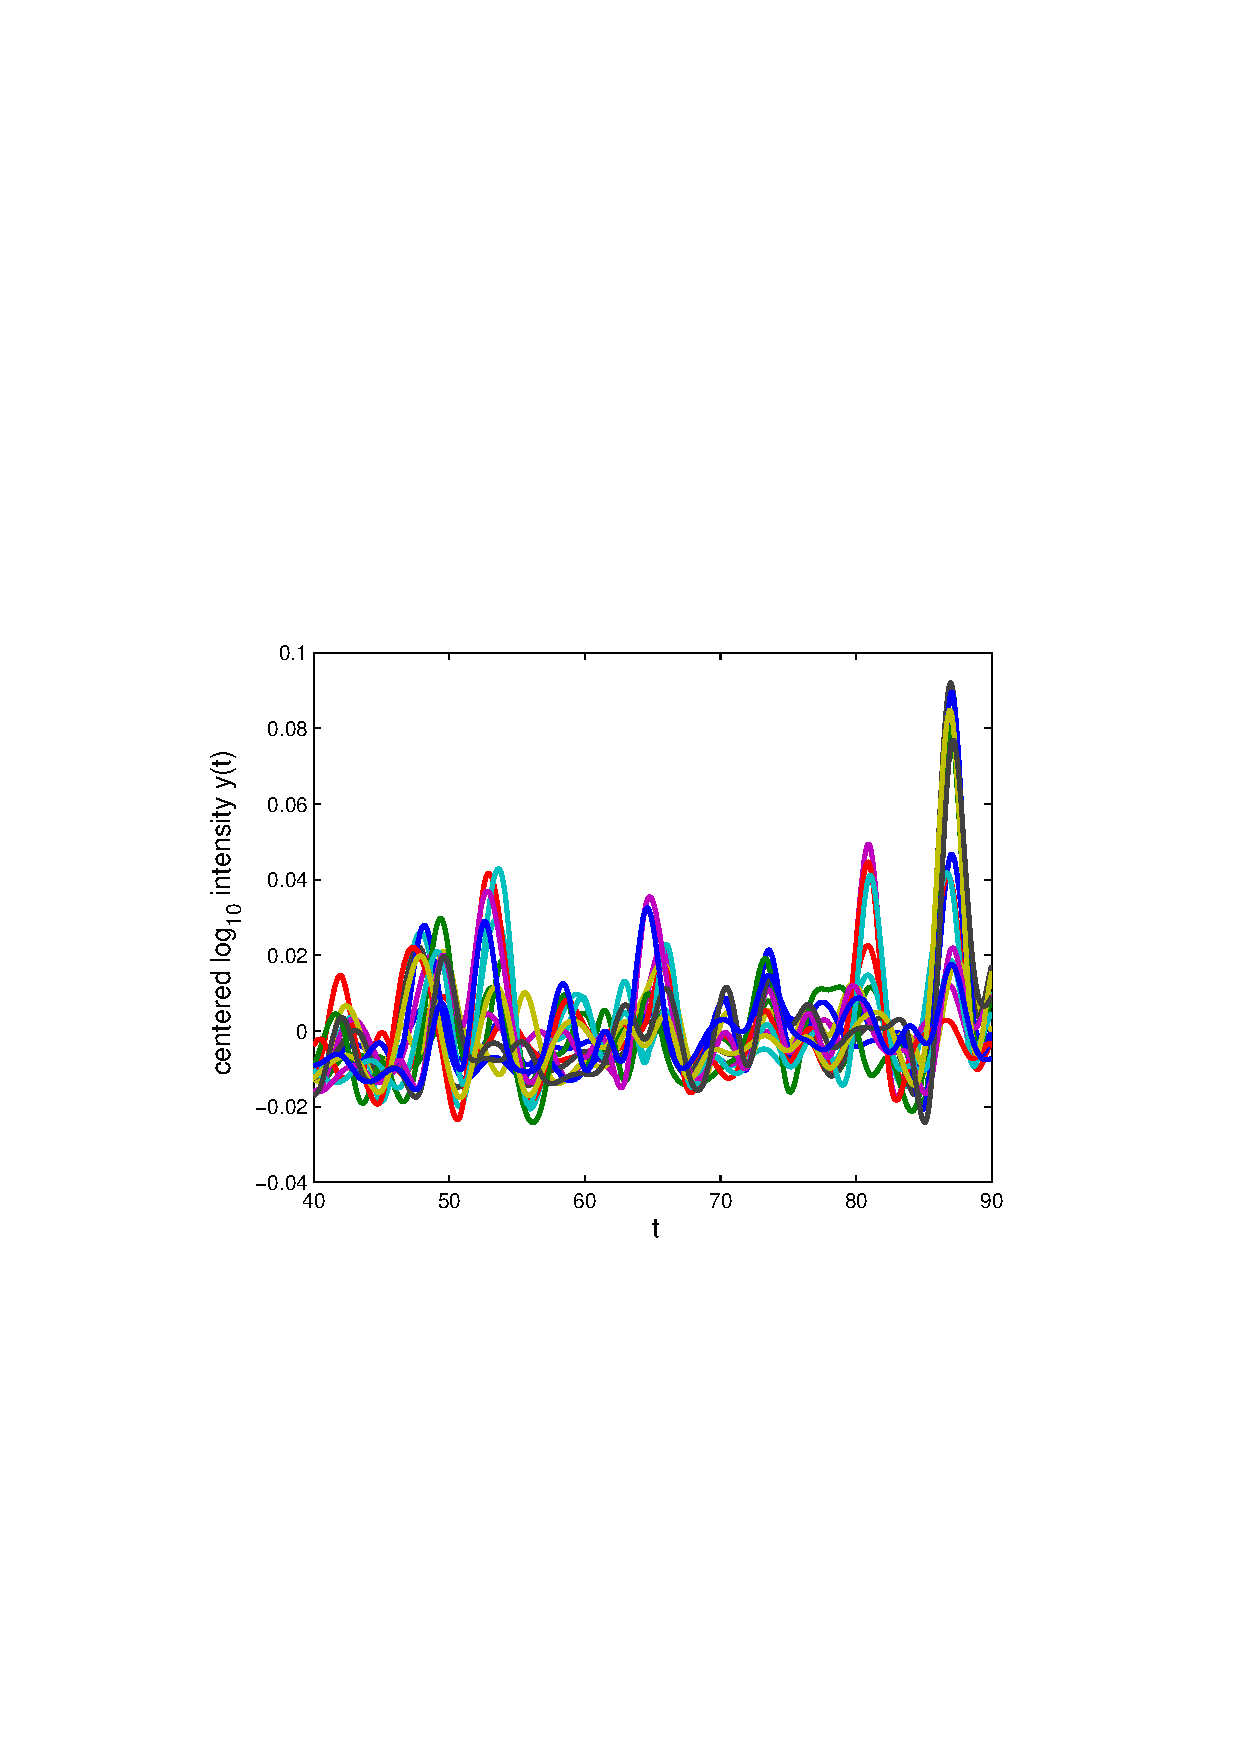
\includegraphics[width=4in]{figs/SelTIC_Ctr.png}
\end{center}

\end{frame}

%  --------------------------------------------------------------------

\begin{frame}

\begin{center}
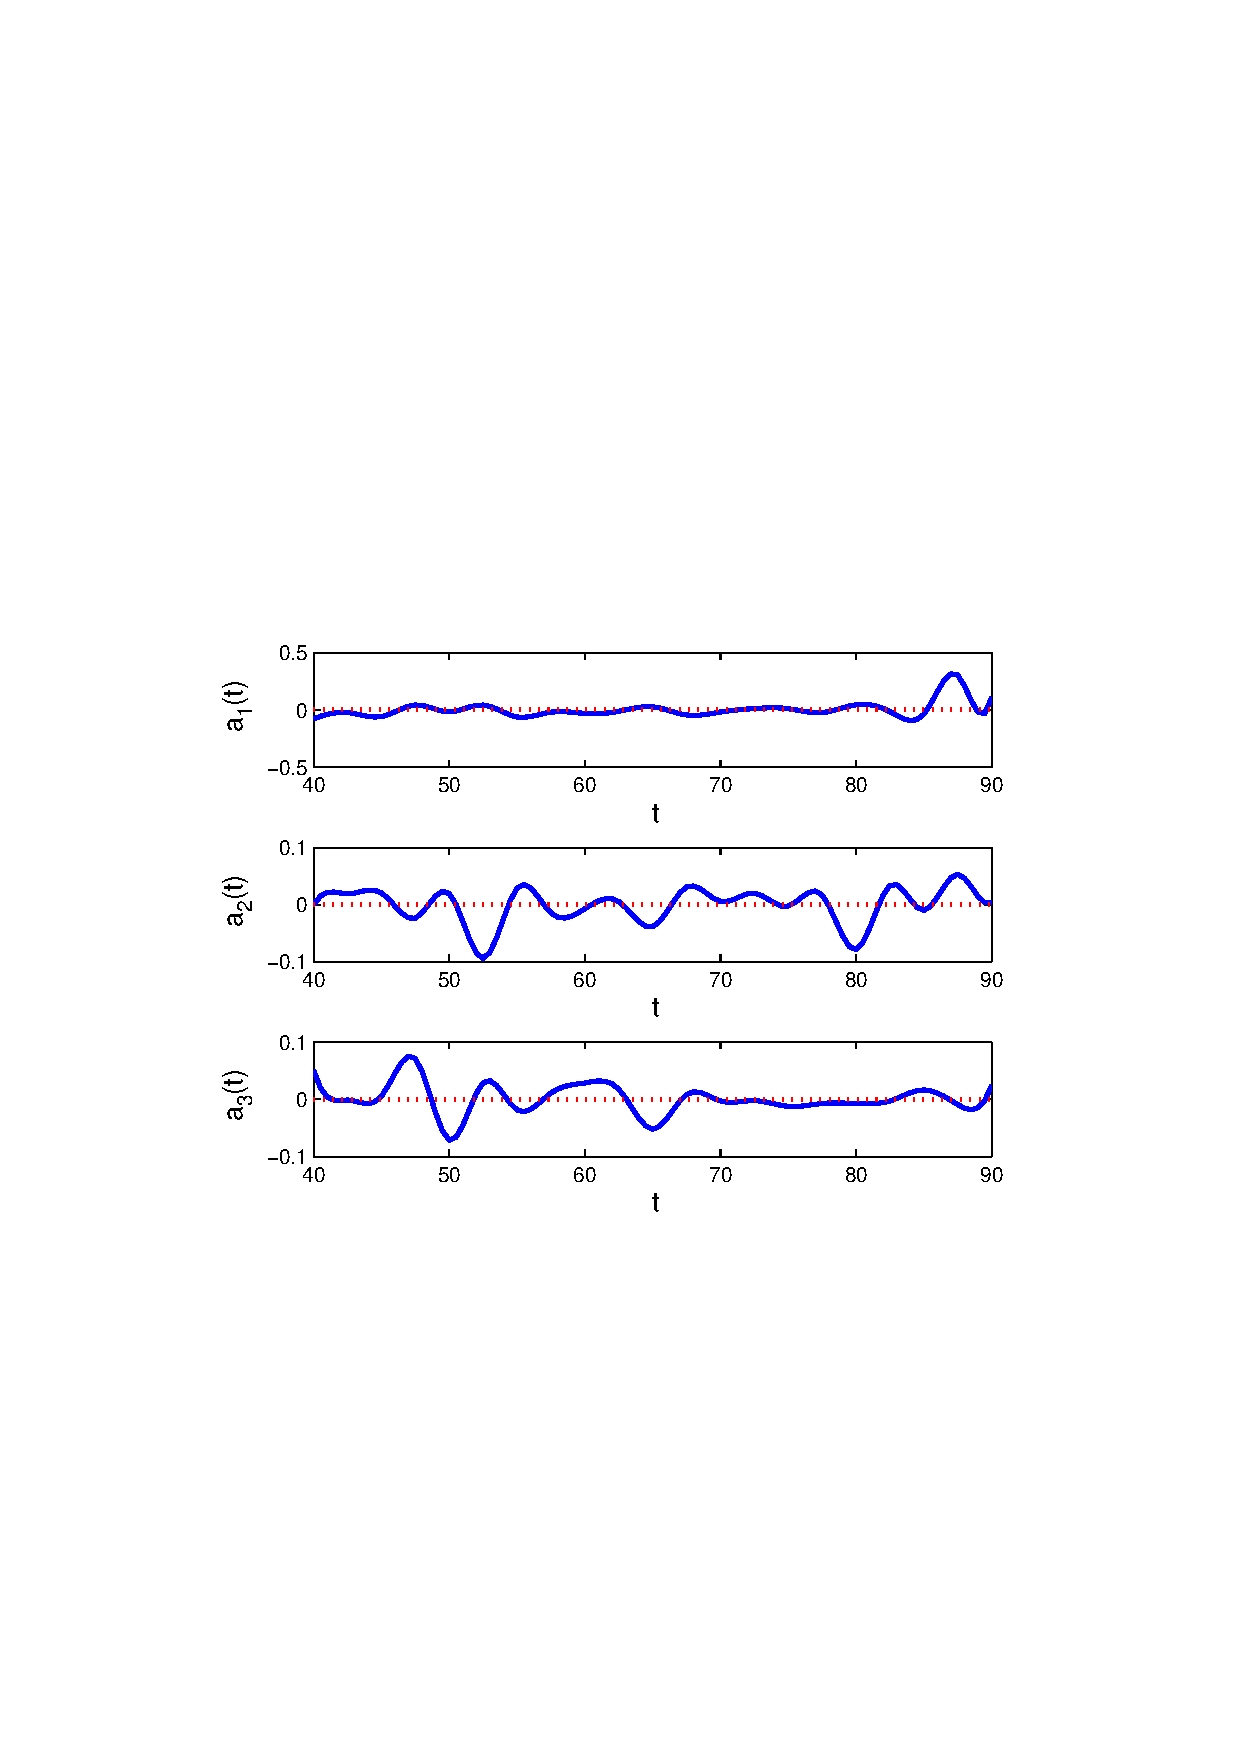
\includegraphics[width=4in]{figs/SelTIC_Coef.png}
\end{center}

\end{frame}

%  --------------------------------------------------------------------

\begin{frame}

\begin{center}
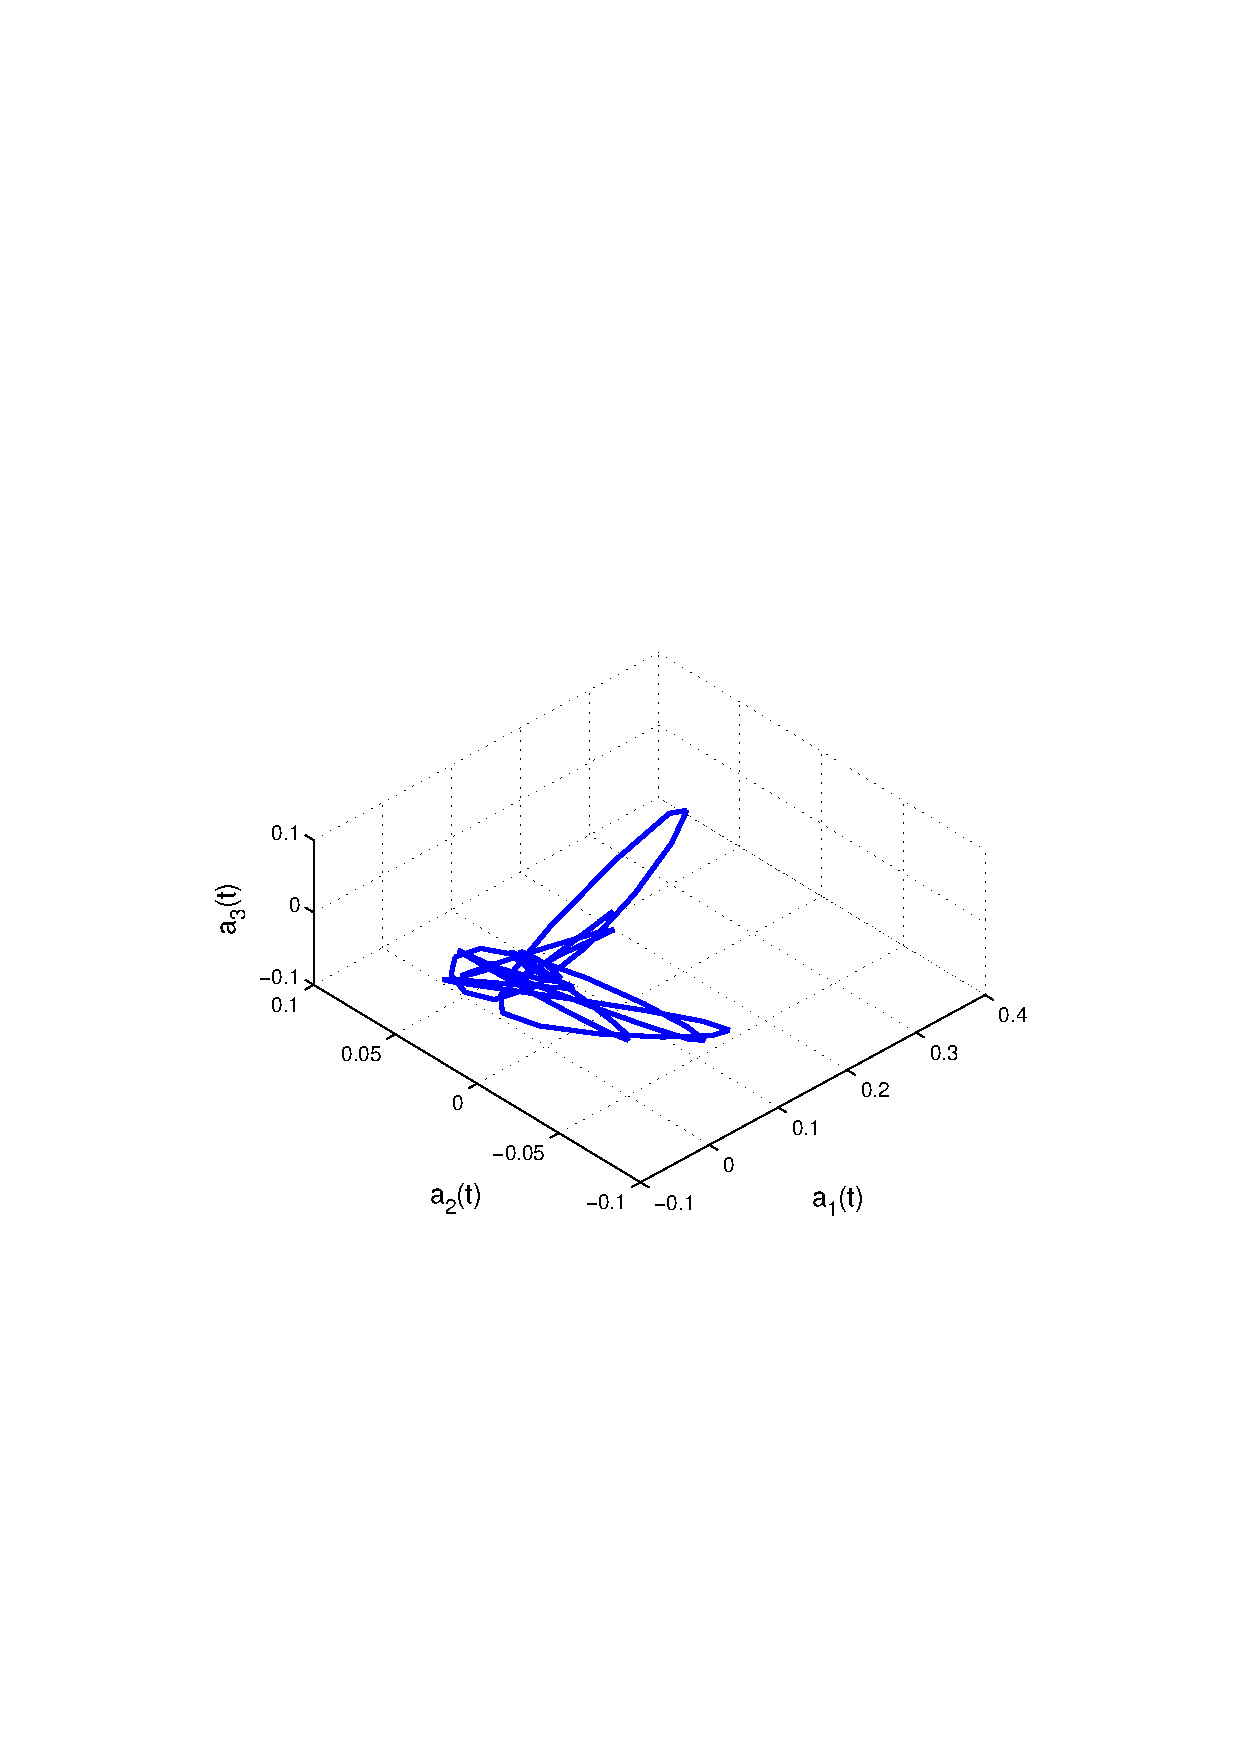
\includegraphics[width=4in]{figs/SelTIC_Coef3d.png}
\end{center}

\end{frame}

%  --------------------------------------------------------------------

\begin{frame}

\begin{center}
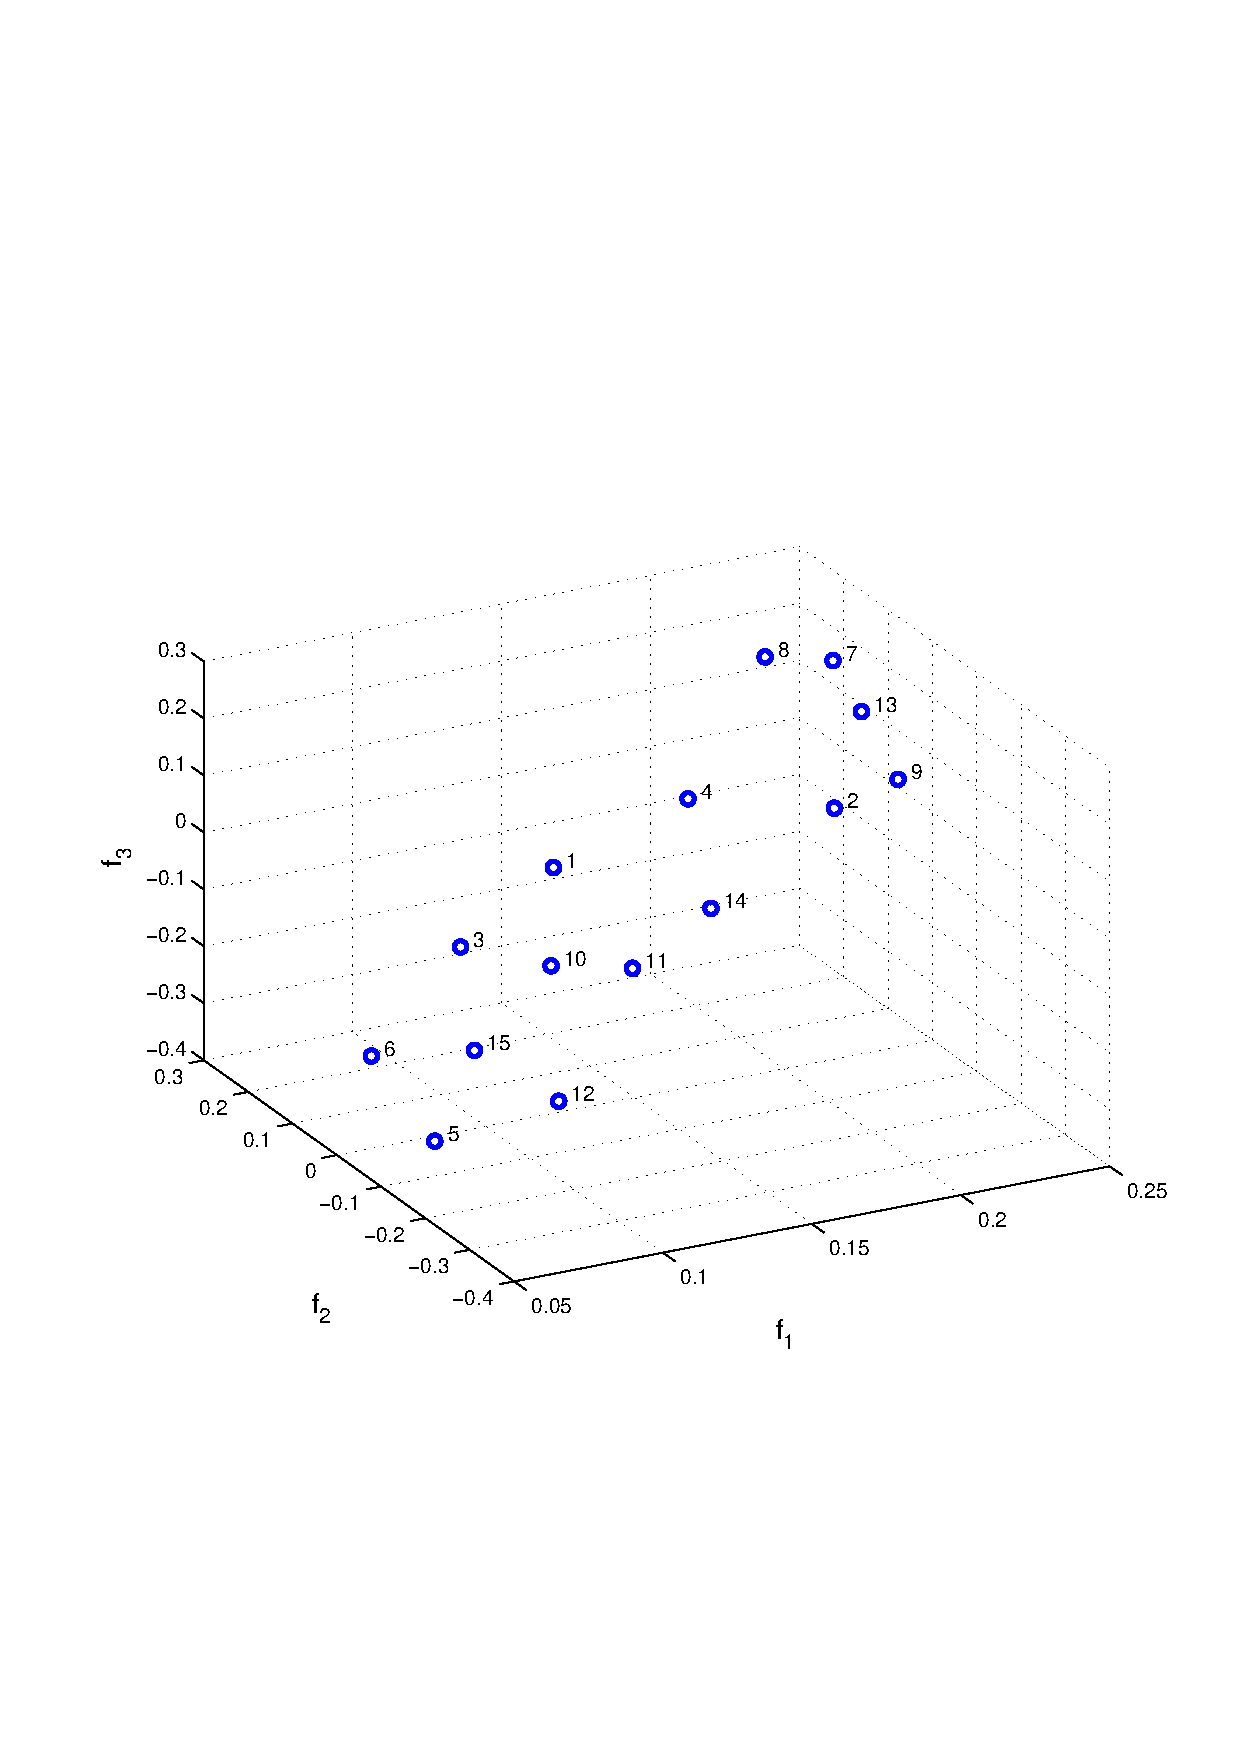
\includegraphics[width=4in]{figs/SelTIC_Scr.png}
\end{center}

\end{frame}

%  --------------------------------------------------------------------

\begin{frame}

\begin{center}
\includegraphics[width=4in]{figs/SelTIC_fit1.png}
\end{center}

\end{frame}

%  --------------------------------------------------------------------

\begin{frame}

\begin{center}
\includegraphics[width=4in]{figs/SelTIC_fit2.png}
\end{center}

\end{frame}

%  --------------------------------------------------------------------

\begin{frame}

\begin{center}
\includegraphics[width=4in]{figs/SelTIC_fit3.png}
\end{center}

\end{frame}

%  --------------------------------------------------------------------

\begin{frame}

\begin{center}
\includegraphics[width=4in]{figs/SelTIC_fit4.png}
\end{center}

\end{frame}

%  --------------------------------------------------------------------

\begin{frame}

\begin{center}
\includegraphics[width=4in]{figs/SelTIC_fit5.png}
\end{center}

\end{frame}

%  --------------------------------------------------------------------

\begin{frame}

\begin{center}
\includegraphics[width=4in]{figs/SelTIC_fit6.png}
\end{center}

\end{frame}

%  --------------------------------------------------------------------

\begin{frame}

\begin{center}
\includegraphics[width=4in]{figs/SelTIC_fit7.png}
\end{center}

\end{frame}

%  --------------------------------------------------------------------

\begin{frame}

\begin{center}
\includegraphics[width=4in]{figs/SelTIC_fit8.png}
\end{center}

\end{frame}

%  --------------------------------------------------------------------

\begin{frame}

\begin{center}
\includegraphics[width=4in]{figs/SelTIC_fit9.png}
\end{center}

\end{frame}

%  --------------------------------------------------------------------

\begin{frame}

\begin{center}
\includegraphics[width=4in]{figs/SelTIC_fit10.png}
\end{center}

\end{frame}

%  --------------------------------------------------------------------

\begin{frame}

\begin{center}
\includegraphics[width=4in]{figs/SelTIC_fit11.png}
\end{center}

\end{frame}

%  --------------------------------------------------------------------

\begin{frame}

\begin{center}
\includegraphics[width=4in]{figs/SelTIC_fit12.png}
\end{center}

\end{frame}

%  --------------------------------------------------------------------

\begin{frame}

\begin{center}
\includegraphics[width=4in]{figs/SelTIC_fit13.png}
\end{center}

\end{frame}

%  --------------------------------------------------------------------

\begin{frame}

\begin{center}
\includegraphics[width=4in]{figs/SelTIC_fit14.png}
\end{center}

\end{frame}

%  --------------------------------------------------------------------

\begin{frame}

\begin{center}
\includegraphics[width=4in]{figs/SelTIC_fit15.png}
\end{center}

\end{frame}

%  --------------------------------------------------------------------

\begin{frame}

\frametitle{Conclusions}

\bi
  \item PCA via eigenanalysis restricts the extendability and versatility of PCA.
  \item Parameter cascading not only regularizes the estimation of nuisance parameters in $\Fbold$,
  \item It re-defines PCA as a much lower dimensional fitting problem.
  \item By treating warping functions as nuisance parameters and defining them as functions of the structural parameters, we can fold registration into PCA and other analyses.
  \item Many other extensions of PCA are made possible as well:
  \bi
    \item GLM models for each variable
    \item Partial least squares fit to an external variable, such as responder/nonresponder for the proteomics data
  \ei
\ei

\end{frame}

\end{document}
